\documentclass{article}
\usepackage{listings}
\usepackage{graphicx}
\usepackage{csquotes}
\usepackage[hidelinks]{hyperref}
%--------------------------------------
\usepackage[utf8]{inputenc}
\usepackage[T1]{fontenc}
%--------------------------------------
%Portuguese-specific commands
%--------------------------------------
\usepackage[portuguese]{babel}
%--------------------------------------
%Hyphenation rules
%--------------------------------------
\usepackage{hyphenat}
\hyphenation{mate-mática recu-perar}
%--------------------------------------
\usepackage{makeidx}
\usepackage[svgnames]{xcolor} % Required to specify font color
\newcommand*{\plogo}{\fbox{$\mathcal{ED}$}} % Generic publisher logo
%----------------------------------------------------------------------------------------
%	TITLE PAGE
%----------------------------------------------------------------------------------------

\newcommand*{\rotrt}[1]{\rotatebox{90}{#1}} % Command to rotate right 90 degrees
\newcommand*{\rotlft}[1]{\rotatebox{-90}{#1}} % Command to rotate left 90 degrees

\newcommand*{\titleBC}{\begingroup % Create the command for including the title page in the document
\centering % Center all text

\def\CP{\textit{\Huge Manual de instruções}} % Title

\settowidth{\unitlength}{\CP} % Set the width of the curly brackets to the width of the title
{\color{LightGoldenrod}\resizebox*{\unitlength}{\baselineskip}{\rotrt{$\}$}}} \\[\baselineskip] % Print top curly bracket
\textcolor{Sienna}{\CP} \\[\baselineskip] % Print title
{\color{RosyBrown}\Large COM EXEMPLOS E ILUSTRAÇÕES} \\ % Tagline or further description
{\color{LightGoldenrod}\resizebox*{\unitlength}{\baselineskip}{\rotlft{$\}$}}} % Print bottom curly bracket

\vfill % Whitespace between the title and the author name

{\Large\textbf{Grupo xy}}\\ % Author name

\vfill % Whitespace between the author name and the publisher logo

\plogo\\[0.5\baselineskip] % Publisher logo
2017 % Year published

\endgroup}


\begin{document}

\pagestyle{empty} % Removes page numbers
\titleBC % This command includes the title page

\pagebreak
\tableofcontents
\pagebreak

\section{Introdução}
Este "manual" serve apenas como um complemento á apresentação e deve ser utilizado juntamente com a cheatsheet. O principal objetivo é dar a conhecer um pouco mais a programação, o arduino e tudo o que se passa em volta disto.

\section{Programação}
A programção é utilizada em praticamente tudo á nossa volta, desde programas para computador, aplicações para smartphones, páginas de internet, robôs, entre muitas outras coisas.\newline \\
Existem várias linguagens diferentes com vários objetivos diferentes. Umas mais rápidas que outras, umas mais leves que outras e todas com formas de se escrever diferente.\newline
Em programação, o primeiro exemplo de código que toda a gente az é o \textit{"Olá mundo!"}. Aqui ficam alguns exemplos em algumas linguagens diferentes:\newline \\
Exemplo em C:
\begin{lstlisting}[language=C]
#include <stdio.h>
#include <stdlib.h>

int main(void)
{
  puts("Hello World!");
  return EXIT_SUCCESS;
}
\end{lstlisting}
\vspace{1em}
Exemplo em Java:
\begin{lstlisting}[language=Java]
class HelloWorld {
  static public void main( String args[] ) {
    System.out.println( "Hello World!" );
  }
}
\end{lstlisting}
\vspace{1em}
Exemplo em Elixir:
\begin{lstlisting}[language=erlang]
defmodule HelloWorld do
  IO.puts "Hello, World!"
end
\end{lstlisting}

\subsection{Controlo}
O controlo baseia-se em condições de acesso que desencadeiam determinadas ações, como por exemplo só quando estiver a pressionar o botão, vai abrir as cortinas da sala, no entanto se tiver a pressionar esse botão não vai iniciar o processo, vai simplesmente deixar que este continue a decorrer. Se eventualmente o botão deixar de ser pressionado então é necessário parar.\newline \\
Essas condições são boleanas, o que significa que apenas são verdadeiras ou falsas.
Normalmente são do tipo \textit{"se (x for verdade) faz (ação y)"} isto se apenas quisermos realizar uma determinada ação quando uma determinada condição for verdade. Se o objetivo for realizar também uma ação quando essa condição for falsa então deve ser algo como \textit{"se (x for verdade) faz (ação y) senão faz (ação z)"}.\newline \\
Mas existe ainda um "senão se" que é usado quando a primeira condição não é verdade mas só se pretende execução a segunda ação dependendo de uma nova condição. Seria algo como \textit{"se (x for verdade) faz (ação y) senão se (h for verdade) faz (ação z)"}. \newline \\
\textbf{Nota}: ver na cheatsheet as instruções para Controlo. \\
\begin{lstlisting}[language=Java]
if(x == 0) {
  y = 3;
}
\end{lstlisting}

\subsection{Operadores}
Os operadores efetuam uma determinada ação que normalmente são realizadas por duas "coisas" do mesmo tipo, ou seja, entre dois numeros ou entre duas (ou mais) letras. Exemplos de operadores são as somas ou subtrações. Por outro lado existem também operadores que são condições como o maior ">" ou menor "<" ou quando é pretendido que duas condições se verifiquem em simultâneo, e então usa-se o operador "e".
\begin{lstlisting}[language=Java]
if(x > 10) {
  terminar();
}
\end{lstlisting}

\begin{figure}[h]
\centering
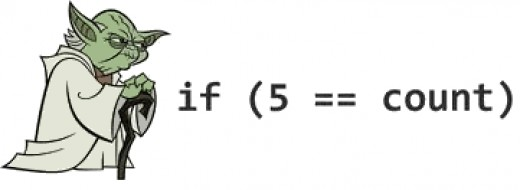
\includegraphics[width=0.5\textwidth]{img/yoda}
\end{figure}

\subsection{Variáveis}
As variáveis servem exencialmente para guardar dados durante a execução de um programa. Esses dados podem ser guardados e utilizados apenas durante um curto espaço de tempo ou durante toda a execução da aplicação.
\begin{lstlisting}[language=Java]
int x = 0;

// faz coisas ...

if(x > 10) {
  terminar();
}
\end{lstlisting}

\section{Scratch}
O scratch é uma plataforma que tem como principal objetivo permitir que pessoas sem qualquer experiencia possam programar. Foi publicado em 2007 sobre a licenca do MIT sendo de livre uso.\newline
Comparativamente á programação utilizado no desenvolvimento de software, o conceito é o mesmo, no entanto as instruções são diferentes.

\begin{figure}[h]
\centering
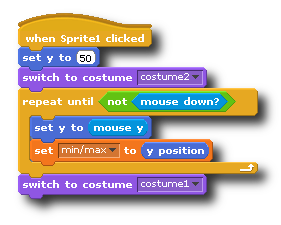
\includegraphics[width=0.5\textwidth]{img/scratch}
\caption{Scratch}
\end{figure}

\section{Arduino}
O arduino é um plataforma de hardware livre que foi projetada com o objetivo de se poder criar prototipos mais rápidamente e mais facilmente. O arduino funciona com linguagem de programação C, e para além disso tem os seu proprios métodos para controlar a entrada e saida de dados da placa, fazendo um tratamento de dados digital e analógico, de forma a facilitar a referida prototipagem.\newline \\
O arduino tornou-se muito famoso por ser fácil de usar mesmo para quem tem muito pouca experiência com programação e mais experiência com eletrónica ou vice-versa, por isso mesmo chegou em especial ao mercado de entusiastas.\newline \\
O arduino provocou também um enorme impulso na cultura maker, pois se até então era necessário ter bons conhecimentos de eletronica e de programação, a partir desse momento tudo se tornou muito mais fácil.\newline \\

\begin{figure}[h]
\centering
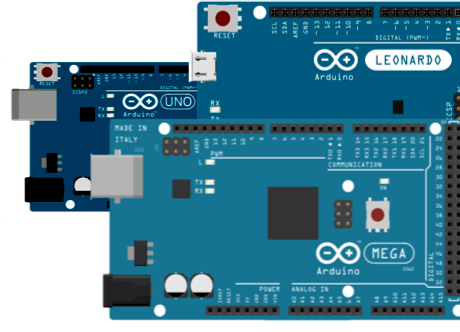
\includegraphics[width=0.5\textwidth]{img/arduino}
\caption{Diferentes modelos de arduino}
\end{figure}

\section{Mais arduino}
Mas o arduino é muito mais que uma simples placa que permite por um LED  piscar. O arduino é uma placa com um microcontrolador, programável, e por isso as opções são ilimitadas. Desde um pequenino carro que evita obstáculos até sistemas que controlam a segurança de edifícios inteiros, utilizando câmeras de vigilância e com sensores de impressões digitais. Ou estufas totalmente autónomas em que a rega depende da humidade do terreno e do ar e depende também do pH da água. Poderia até utilizar-se um sistema de inteligência artificial que ia aprendendo de acordo com o tratamento que fazia, comparando com os resultados. As opções são infinitas.

\subsection{Módulos}
Os módulos são um conjunto de componentes já conectados numa placa, desenvolvidos com um determinado objetivo. Exemplos de módulos são :
\begin{enumerate}
\item WiFi
\item GPS
\item GPRS
\item RFID
\end{enumerate}

\begin{figure}[h]
\centering
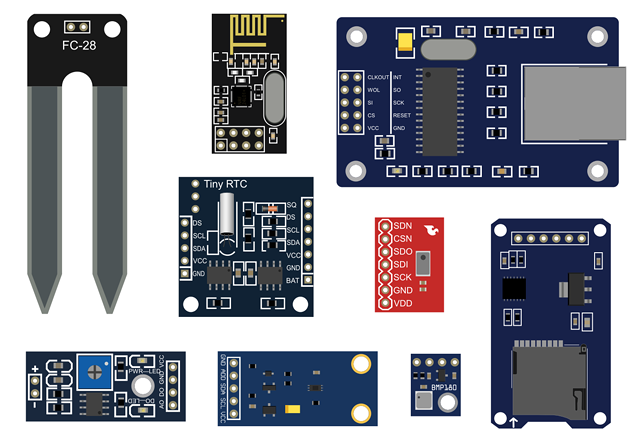
\includegraphics[width=0.65\textwidth]{img/shields}
\caption{Módulos}
\end{figure}

\subsection{Datasheets}
Como é que sabemos as propriedas de um determinado objeto que queremos comprar? Se precisamos de soldar um componente mas não soubermos que temperatura é que ele suporta (demasiado calor poder danificar parcialmente ou totalmente o componente), ou se precisarmos de saber mais sobre esse componente.\newline \\
Os datasheets contêm toda essa informação. Normalmente são feitos por quem desenvolve o componente e neles deve haver informação suficiente para que qualquer pessoa que compre esse componente, encontre as respostas às suas dúvidas no respetivo datasheet.\newline \\
Um exemplo de um datasheet pode ser encontrado em \url{http://www.midondesign.com/Documents/LM78L05.PDF}, que corresponde a um regulador de tensão.

\section{Movimento Maker}
O \textit{movimento maker} é uma ideia que tem atraido cada vez mais pessoas. Existem páginas online, grupos nas redes sociais, cada vez mais pessoas tem aderido. Essa aderencia deve-se ao facto de o arduino ter facilitado muito a prototipagem e por isso, os primeiros interessados foram os programadores, que já com conhecimento de programação, quiseram explorar um pouco o mundo de eletronica, mecatronica, robotica, etc.\newline
Á medida que mais pessoas se foram juntados, houve mais pessoas a partilhar os seus trabalhos e cada vez trona-se mais fácil encontrar exemplos e fazer algo.

\begin{figure}[h]
\centering
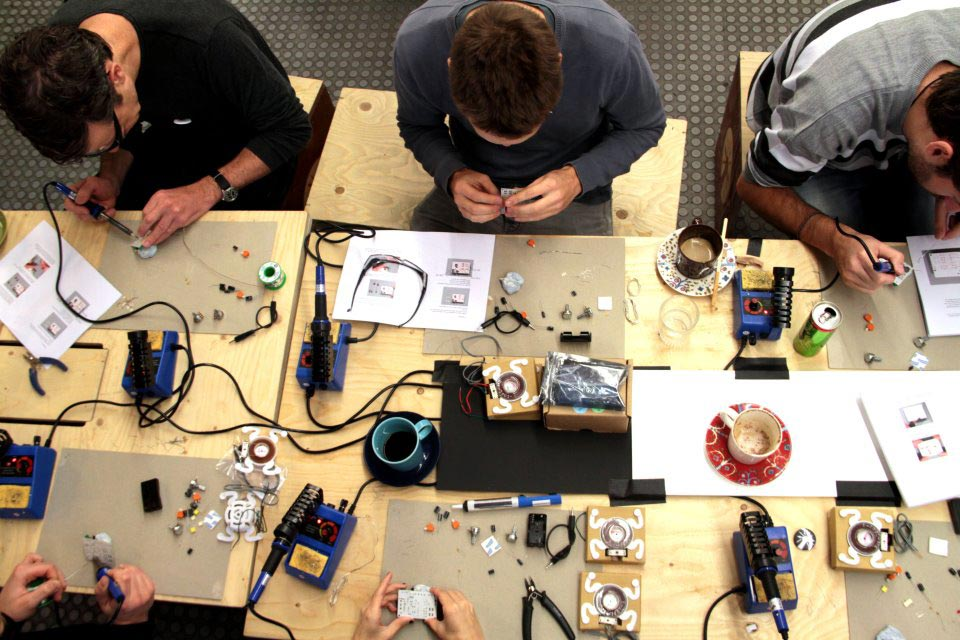
\includegraphics[width=0.8\textwidth]{img/makers}
\caption{Movimento maker}
\end{figure}

\subsection{Maker Faire Lisboa}
Com tanta aderencia a este movimento começaram a surgir eventos. Um deles é a \textit{Maker Fair Lisboa} que junta centenas de pessoas todos os anos. É possivel encontrar todos os tipos de projetos DIY (\textit{Do it Yourself} - Faça você mesmo) nas mais variadas áreas, desde projetos ligados ao ambiente até projetos desenvolvidos apenas por diversão.

\begin{figure}[h]
\centering
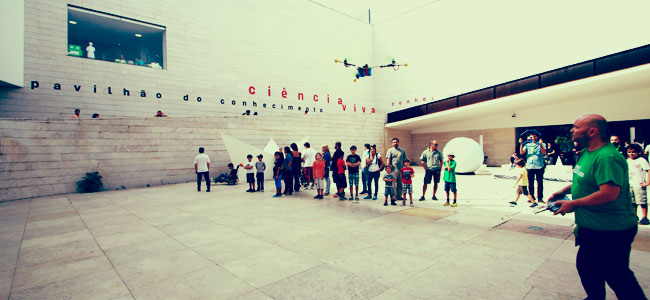
\includegraphics[width=0.8\textwidth]{img/mflisboa}
\caption{Maker Faire Lisboa}
\end{figure}

\section{Links úteis}
\url{https://www.arduino.cc/}\newline
\url{https://www.arduino.cc/en/Reference/HomePage}\newline
\url{https://www.arduino.cc/en/Tutorial/HomePage}\newline\newline
\url{https://www.adafruit.com/}\newline
\url{https://learn.adafruit.com/}\newline

% link para testes (Pedro)

\section{Exemplos}
% TODO exemplos em scratch e traduzidos para c

\section{Conclusão}
Esperamos que tenham gostado deste workshop, tenham aprendido coisas novas e acima de tudo, que se tenham divertido.
Se quiserem obter mais informações contactem a nossa página fb.me/arduinosolidario

\end{document}
